\begin{figure}[t]%
  \centering
  \begin{subfigure}{\textwidth}
    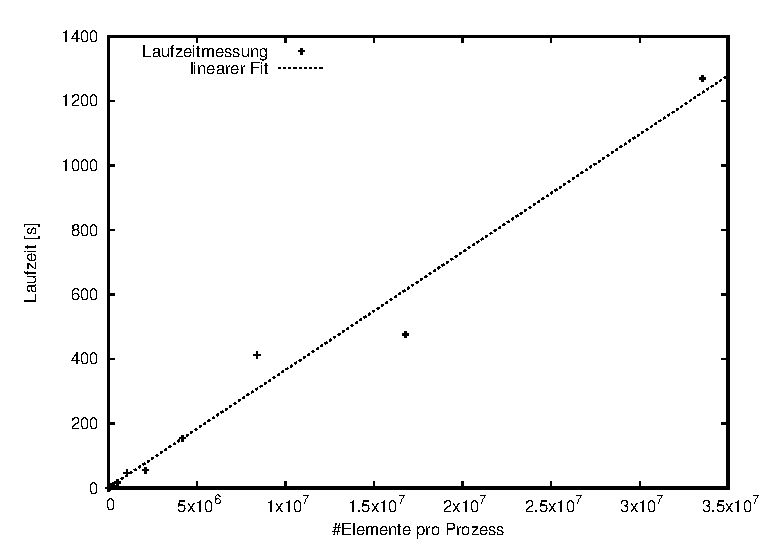
\includegraphics[width=0.8\textwidth]{img/grav1_lin.eps}
    \subcaption{Dieser Testlauf wurde mit $p = 1$ durchgeführt und entspricht damit der nicht-parallelen Variante.}
  \end{subfigure}
  \begin{subfigure}{\textwidth}
    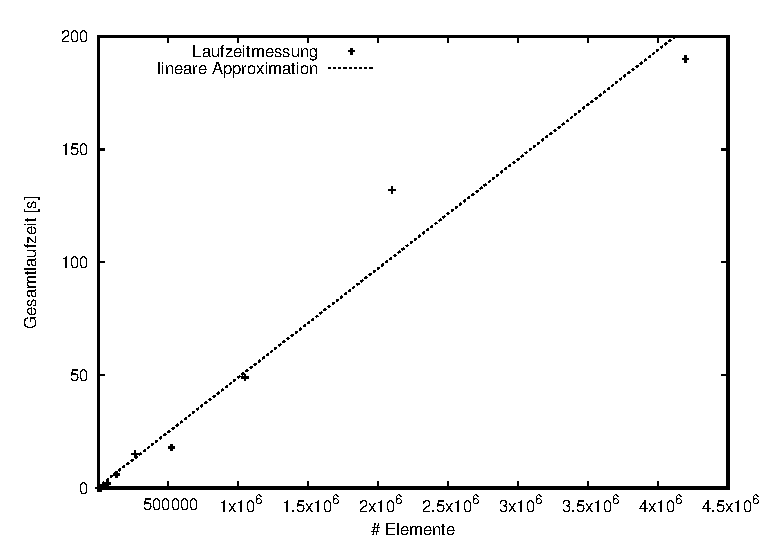
\includegraphics[width=0.8\textwidth]{img/grav_32_lin.eps}
    \subcaption{Dieser Testlauf wurde mit $p = 32$ durchgeführt, genau ein Knoten des Rechenclusters auszulasten.}
  \end{subfigure}
  \caption{In dieser Abbildung ist der Zusammenhang der Laufzeit mit der Anzahl an Elementen pro Prozess dargestellt.}
  \label{fig:1-32x}
\end{figure}